%%%%%%%%%%%%%%%%%%%%%%%%%%%%%%%%%%%%%%%%%%%%%%%%%%%%%%%%%%%%%%%%%%%%%%%%
%
% Template latex file for a common article class for class notes
% and write ups. Additional Configuration and styling options are 
% commented out. ex. Table of Contents and Title page
% 
% Author: Amy Bui
% 
%%%%%%%%%%%%%%%%%%%%%%%%%%%%%%%%%%%%%%%%%%%%%%%%%%%%%%%%%%%%%%%%%%%%%%%%
 
\documentclass[12pt]{article}
\usepackage[utf8]{inputenc}
\usepackage{parskip}
\usepackage{tabularx}
\usepackage{array}
\usepackage{appendix}
% \usepackage[showframe=true]{geometry}
\usepackage{changepage}
% \usepackage{csvsimple}
% \usepackage[framemethod=tikz]{mdframed}
% \usepackage[color, leftbars]{changebar}
% \usepackage[inkscapeformat=png]{svg}
% \usepackage{svg}
% \usepackage[inkscape={/Applications/Inkscape.app/Contents/Resources/bin/inkscape -z -C}]{svg}

% Important Configurations
 
%%%%%%%%%%%%%%%%%%%%%%%%%%%%%%%%%%%%%%%%%%%%%%%%%%%%%%%%%%%%%%%%%%%%%%%%
% Reduce margin
%
% \addtolength{\oddsidemargin}{-.85in}
% \addtolength{\evensidemargin}{-.85in}
% \addtolength{\textwidth}{1in}

% \addtolength{\topmargin}{-.85in}
% \addtolength{\textheight}{1in}

% Page format commands:
% Override normal article margins,
% making the margins smaller
\setlength{\textwidth}{6.5in}
\setlength{\textheight}{9in}
\setlength{\oddsidemargin}{0in}
\setlength{\evensidemargin}{0in}
\setlength{\topmargin}{-0.6in}

\setlength{\parindent}{0pt}
%%%%%%%%%%%%%%%%%%%%%%%%%%%%%%%%%%%%%%%%%%%%%%%%%%%%%%%%%%%%%%%%%%%%%%%%


%%%%%%%%%%%%%%%%%%%%%%%%%%%%%%%%%%%%%%%%%%%%%%%%%%%%%%%%%%%%%%%%%%%%%%%%
% Math Symbols
\usepackage{mathtools}
\usepackage{amssymb}
% \usepackage{epsfig}
\usepackage{amsmath,amsthm}
\usepackage{amscd,amsxtra,latexsym}


% add floor and ceiling symbol. Usage: \ceil*{}, \floor*{}
\DeclarePairedDelimiter\ceil{\lceil}{\rceil}
\DeclarePairedDelimiter\floor{\lfloor}{\rfloor}

% multiset \langle ... \rangle
\def\multiset#1#2{\ensuremath{\left(\kern-.3em\left(\genfrac{}{}{0pt}{}{#1}{#2}\right)\kern-.3em\right)}}



%%%%%%%%%%%%%%%%%%%%%%%%%%%%%%%%%%%%%%%%%%%%%%%%%%%%%%%%%%%%%%%%%%%%%%%%

%%%%%%%%%%%%%%%%%%%%%%%%%%%%%%%%%%%%%%%%%%%%%%%%%%%%%%%%%%%%%%%%%%%%%%%%
% Code Sample Styling

% use \lstinline! xxx ! or \begin{lstlisting} ... \end{lstlisting}
\usepackage{listings}

\usepackage{color}
\definecolor{light-gray}{gray}{0.97} % shade of grey
\definecolor{dkgreen}{rgb}{0,0.6,0}
\definecolor{gray}{rgb}{0.5,0.5,0.5}
\definecolor{mauve}{rgb}{0.58,0,0.82}

% \begin{lstlisting}[...] ... \end{lstlisting}
\lstset{frame=none,
    language=Verilog,
    aboveskip=3mm,
    belowskip=3mm,
    stepnumber=0, % set to 0 if you don't like line nums
    showstringspaces=false,
    columns=flexible,
    basicstyle={\small\ttfamily},
    numbers=left,
    numberstyle=\color{black},
    keywordstyle=\color{blue},
    commentstyle=\color{dkgreen},
    stringstyle=\color{mauve},
    backgroundcolor=\color{light-gray},
    breaklines=true,
    breakatwhitespace=false,
    tabsize=2
}

% \newcommand\mylstcaption{}

% \mdfdefinestyle{mymdstyle}{
% hidealllines=true,
% middleextra={
%   \node[anchor=west] at (O|-P)
%     {\lstlistingname~\thelstlisting\  (Cont.):~\mylstcaption};},
% secondextra={
%   \node[anchor=west] at (O|-P)
%     {\lstlistingname~\thelstlisting\  (Cont.):~\mylstcaption};},
% splittopskip=2\baselineskip
% }

% \surroundwithmdframed[style=mymdstyle]{lstlisting}
% \newmdenv[style=mymdstyle]{mdlisting}



%%%%%%%%%%%%%%%%%%%%%%%%%%%%%%%%%%%%%%%%%%%%%%%%%%%%%%%%%%%%%%%%%%%%%%%%

%%%%%%%%%%%%%%%%%%%%%%%%%%%%%%%%%%%%%%%%%%%%%%%%%%%%%%%%%%%%%%%%%%%%%%%%
\usepackage{xcolor}
%% https://tex.stackexchange.com/questions/401750/quick-and-short-command-for-coloring-one-word
\newcommand\shorthandon{\catcode`@=\active \catcode`^=\active \catcode`*=\active }
\newcommand\shorthandoff{\catcode`@=12 \catcode`^=7 \catcode`*=12 }
\shorthandon
\def@#1@{\textcolor{red}{#1}}%
\def^#1^{\textcolor{blue}{#1}}%
\def*#1{\string#1}
\shorthandoff
%% useage: \textcolor{red}{text here}
% \shorthandon
% This is a @test@ of the ^emergency^ bro*@dcast system.
% \shorthandoff
%%%%%%%%%%%%%%%%%%%%%%%%%%%%%%%%%%%%%%%%%%%%%%%%%%%%%%%%%%%%%%%%%%%%%%%%


%%%%%%%%%%%%%%%%%%%%%%%%%%%%%%%%%%%%%%%%%%%%%%%%%%%%%%%%%%%%%%%%%%%%%%%%

%Commands below change page margins (this much space at the titlepage, etc)
\newlength{\toppush}
\setlength{\toppush}{2\headheight}
\addtolength{\toppush}{\headsep}

% Section header Styling
% The commands below change the bold text where it says "Section" into "Question"
% \usepackage{titlesec}
% \titleformat{\section}
% {\normalfont\Large\bfseries}{Question~\thesection:}{1em}{}

% I added this command below to chance "subsections numbers" to be "Question [subsection number]" -AB 1/31/2021
% \titleformat{\subsection}
% {\normalfont\bfseries}{\thesubsection:}{1em}{}

% Page head Styling
% Name and subject of the class
\def\subjnum{EE 156}          % Class Number
\def\subjname{Advance Topics in Computer Architecture}       % Class Name

% Name of the student, university name and which semester
\def\doheading#1#2#3{\vfill\eject\vspace*{-\toppush}%
  \vbox{\hbox to\textwidth{{\bf} \subjnum: \subjname \hfil Amy Bui}%
    \hbox to\textwidth{{\bf} Tufts University, Spring 2023 \hfil#3\strut}%
    \hrule}}

%Command for the title of the document (Homework 0)
\newcommand{\htitle}[1]{\vspace*{1.25ex plus 1ex minus 0ex}%
\begin{center}
    {\large\bf #1}
\end{center}} 
%%%%%%%%%%%%%%%%%%%%%%%%%%%%%%%%%%%%%%%%%%%%%%%%%%%%%%%%%%%%%%%%%%%%%%%%



%%%%%%%%%%%%%%%%%%%%%%%%%%%%%%%%%%%%%%%%%%%%%%%%%%%%%%%%%%%%%%%%%%%%%%%%
% Misc
\usepackage{graphicx} % graphics
\usepackage{enumitem} % listing style (bullet lists)

% below helps with trying to get figures in a row
\usepackage{caption}
\usepackage{subcaption}

% hyperlink styling
% use \href{} and \url{}, and colors table of contents links
% use \href{} and \url{}
% \label{sec:name}
% \hyperref[label]{text}
\usepackage{hyperref}
\hypersetup{
    colorlinks=true,
    linkcolor=blue, % was previously black
    filecolor=magenta,
    urlcolor=blue,
    pdftitle={Template}
}
\urlstyle{same}

% A command for primes (')
\newcommand{\p}%
    {\ensuremath{^{\prime}}}

% a command for double primes ('')
\newcommand{\pp}%
    {\ensuremath{^{\prime \prime}}}

% A command for the Kleene star
\newcommand{\str}%
    {\ensuremath{^{\star}}}

% a command for the double star
\newcommand{\sstr}%
    {\ensuremath{^{\star\star}}}
%%%%%%%%%%%%%%%%%%%%%%%%%%%%%%%%%%%%%%%%%%%%%%%%%%%%%%%%%%%%%%%%%%%%%%%%

% Options for title page, use \maketitle in document
% \author{Amy Bui}
% \title{COMP160 - Algorithms: Class Notes and Practice}


\begin{document}
%% create title page
% \title{(g)ROOT \\ Language Reference Manual}
% \author{Samuel Russo \quad Amy Bui \quad Eliza Encherman \\ Zachary Goldstein \quad Nickolas Gravel}
% \date{\today}
% \maketitle

\doheading{2}{title}{Lab 0}

    %%%%%%%%%%%%%%%%%%%%%%%%%%%%%%%%%%%%%%%%%%%%%%%%%%%%%%%%%%%%%%%%%%%%%%%%
    % Table of Contents
    \setcounter{tocdepth}{2}
    \tableofcontents
    % \pagebreak
    %%%%%%%%%%%%%%%%%%%%%%%%%%%%%%%%%%%%%%%%%%%%%%%%%%%%%%%%%%%%%%%%%%%%%%%%

    \begin{thebibliography}{1}
        \bibitem[1]{sniper}\href{https://snipersim.org/w/The_Sniper_Multi-Core_Simulator}{The Sniper Multi-Core Simulator}
        \bibitem[2]{parallel}O. Tange (2011): \href{https://www.gnu.org/software/parallel/parallel_tutorial.html}{GNU Parallel}  - The Command-Line Power Tool
        \bibitem[3]{oh}Mark, Robert, and Bharat's office hours
        \bibitem[4]{splash2}S. C. Woo, M. Ohara, E. Torrie, J. P. Singh and A. Gupta, \href{https://citeseerx.ist.psu.edu/viewdoc/download?doi=10.1.1.48.2356&rep=rep1&type=pdf}{The SPLASH-2 Programs: Characterizaion and Methodological Considerations}, Proceedings 22nd Annual International Symposium on Computer Architecture, Santa Margherita Ligure, Italy, 1995, pp. 24-36
        \bibitem[5]{book}John L. Hennessy and David A. Patterson. 2017. Computer Architecture, Sixth Edition: A Quantitative Approach (6th. ed.). Morgan Kaufmann Publishers Inc., San Francisco, CA, USA.
    \end{thebibliography}

    \section{Intro}
        The purpose of this experiement is to sweep different test applications (benchmarks) across different configurations of L2 cache sizes, in order to learn the \texttt{SniperSim} tool. We analyze the affects of L2 cache sizes on instructions per clock cycle (IPC) and energy consumption. It is observed that as L2 cache size increases, total energy consumption of a test application also increases slightly, but the L2 energy consumption increases more noticeably. L2 cache size also affects performance (measured by IPC here) differently depending on how much time a process spends on certain types of instructions; L2 cache size is likely to affect IPC if a benchmark substantially relied on memory access operations. 

        
    \clearpage

    \section{Experimental Setup}

        Nine simulations run for an x86 architecture simulator, Sniper 7.3 \cite{sniper}. They are simulated with three \texttt{splash2} benchmarks: \texttt{fft\_O2}, \texttt{ocean.cont}, and \texttt{radix}\cite{splash2}. Each were configured with the same L1 cache size (32 KB) and configuration values set in the \texttt{gainestown.cfg}. Differing L2 cache size topologies (configurations) were tested with the three test applications: 512 KB, 1 MB, and 4 MB (See Fig. 9 of Lab 0 Specification). Input size used for all tests was preset \texttt{small}. Figure \ref{topology} visualizes the topology for simulations using 512 KB L2 cache; the configuration is the same across the other simulations, only differing in what is labeled for L2 size. To note: L2 cache associativity is 8 and cache block size is 64 bytes across all simulations, given by \texttt{gainestown}.

        Simulations ran concurrently using bash script(s) and GNU \texttt{parallel} shell tool\cite{parallel}, and post processing of the data were handled with python (v2.7) and bash scripts (included separately). Simulations ran on a python virtual environment and in a detached \texttt{tmux} session, due to long duration of the experiments. Sniper provided data processing tools used were: \texttt{gen\_topology.py}, \texttt{cpi-stack.py}, and \texttt{mcpat.py}.

    % \clearpage

        \begin{figure}[hbt!] 
            \centering
            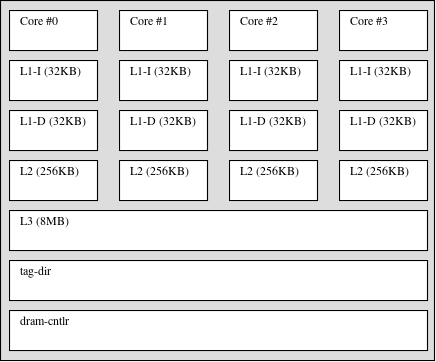
\includegraphics[width=0.6\textwidth]{output/fft_O2/lab0L2-512KB/topo.png}
            \caption{Topology for \texttt{fft\_O2}, \texttt{ocean.cont}, and \texttt{radix} benchmark tests with 512 KB L2 cache size (topologies for the 1 MB and 4 MB L2 (marked red dot) tests are the same). All benchmarks were run in \texttt{Sniper-7.3} with the \texttt{gainestown} configuration using the \texttt{--viz} and \texttt{--roi} options.}
            \label{topology}
        \end{figure}

        
    \clearpage
    %%%%%%%%%%%%%%%%%%%%%%%%%%%%%%%%%%%%%%%%%%%%%%%%%%%%%%%%%%%%%%%%%%%%%%%%


    \section{Energy Results}
    % \lstinputlisting{hello.c}

    The following discusses the energy and cpi stacks for common L2 cache sized benchmarks. For post processed data, see Fig. \ref{fig:fftO2:power}, Fig. \ref{fig:ocean.cont:power}, and Fig. \ref{fig:radix:power} for the energy stacks of core 0 of the benchmarks \texttt{fft\_O2}, \texttt{ocean.cont}, and \texttt{radix}, respectively, and Fig. \ref{fig:fftO2:cpi-stack}, Fig. \ref{fig:ocean.cont:cpi-stack}, and Fig. \ref{fig:radix:cpi-stack} for the corresponding CPI stacks. Specific values are also in the Appendix for each stack. We analyze the pattern in the following stacks (color legend at the end):

    \begin{figure}[hbt!]
        \centering
        \begin{adjustwidth}{-2.5cm}{}
        \begin{tabular}{ccc}
            \begin{subfigure}{0.4\textwidth}
                \centering
                \includegraphics[width=1\textwidth]{output/fft_O2/lab0L2-512KB/power-chop.png}
                \caption{\texttt{fft\_O2}: L2 enery 0.03 J; Total energy 0.53 J}
                \label{fig512KBcompare.fft:power}
            \end{subfigure} &
            \begin{subfigure}{0.4\textwidth}
                \centering
                \includegraphics[width=1\textwidth]{output/ocean.cont/lab0L2-512KB/power-chop.png}
                \caption{\texttt{ocean.cont}: L2 energy 0.15 J; Total energy 2.03 J}
                \label{fig512KBcompare.ocean.cont:power}
            \end{subfigure} & 
            \begin{subfigure}{0.4\textwidth}
                \centering
                \includegraphics[width=1\textwidth]{output/radix/lab0L2-512KB/power-chop.png}
                \caption{\texttt{radix}: L2 energy 0.04 J; Total energy 0.34 J}
                \label{fig512KBcompare.radix:power}
            \end{subfigure} \\
            \begin{subfigure}{0.4\textwidth}
                \centering
                \includegraphics[width=1\textwidth]{output/fft_O2/lab0L2-512KB/cpi-stack-chop.png}
                \caption{\texttt{fft\_O2}}
                \label{fig512KBcompare.fft:cpi}
            \end{subfigure} &
            \begin{subfigure}{0.4\textwidth}
                \centering
                \includegraphics[width=1\textwidth]{output/ocean.cont/lab0L2-512KB/cpi-stack-chop.png}
                \caption{\texttt{ocean.cont}}
                \label{fig512KBcompare.ocean:cpi}
            \end{subfigure} & 
            \begin{subfigure}{0.4\textwidth}
                \centering
                \includegraphics[width=1\textwidth]{output/radix/lab0L2-512KB/cpi-stack-chop.png}
                \caption{\texttt{radix}}
                \label{fig512KBcompare.radix:cpi}
            \end{subfigure}
        \end{tabular}
        \end{adjustwidth}
        \caption{\textbf{512 KB L2 Cache Size:} Energy stacks for (a,d) \texttt{fft\_O2}, (b,e) \texttt{ocean.cont}, and (c.f) \texttt{radix} benchmarks using \textbf{512 KB} L2 cache size on core 0, and their corresponding CPI stacks.}
        \label{fig512KBcompare}
    \end{figure}
    % \clearpage

    \begin{figure}[hbt!]
        \centering
        \begin{adjustwidth}{-2.5cm}{}
        \begin{tabular}{ccc}
            \begin{subfigure}{0.4\textwidth}
                \centering
                \includegraphics[width=1\textwidth]{output/fft_O2/lab0L2-1MB/power-chop.png}
                \caption{\texttt{fft\_O2}: L2 energy 0.07 J; Total energy 0.57 J}
                \label{fig1MBcompare.fft:power}
            \end{subfigure} &
            \begin{subfigure}{0.4\textwidth}
                \centering
                \includegraphics[width=1\textwidth]{output/ocean.cont/lab0L2-1MB/power-chop.png}
                \caption{\texttt{ocean.cont}: L2 energy 0.30 J; Total energy 2.11 J}
                \label{fig1MBcompare.ocean.cont:power}
            \end{subfigure} & 
            \begin{subfigure}{0.4\textwidth}
                \centering
                \includegraphics[width=1\textwidth]{output/radix/lab0L2-1MB/power-chop.png}
                \caption{\texttt{radix}: L2 energy 0.08 J; Total energy 0.38 J}
                \label{fig1MBcompare.radix:power}
            \end{subfigure} \\
            \begin{subfigure}{0.4\textwidth}
                \centering
                \includegraphics[width=1\textwidth]{output/fft_O2/lab0L2-1MB/cpi-stack-chop.png}
                \caption{\texttt{fft\_O2}}
                \label{fig1MBcompare.fft:cpi}
            \end{subfigure} &
            \begin{subfigure}{0.4\textwidth}
                \centering
                \includegraphics[width=1\textwidth]{output/ocean.cont/lab0L2-1MB/cpi-stack-chop.png}
                \caption{\texttt{ocean.cont}}
                \label{fig1MBcompare.ocean:cpi}
            \end{subfigure} & 
            \begin{subfigure}{0.4\textwidth}
                \centering
                \includegraphics[width=1\textwidth]{output/radix/lab0L2-1MB/cpi-stack-chop.png}
                \caption{\texttt{radix}}
                \label{fig1MBcompare.radix:cpi}
            \end{subfigure}
        \end{tabular}
        \end{adjustwidth}
        \caption{\textbf{1 MB L2 Cache Size:} Energy stacks for (a,d) \texttt{fft\_O2}, (b,e) \texttt{ocean.cont}, and (c.f) \texttt{radix} benchmarks using \textbf{1 MB} L2 cache size on core 0, and their corresponding CPI stacks.}
        \label{fig1MBcompare}
    \end{figure}

    \begin{figure}[hbt!]
        \centering
        \begin{adjustwidth}{-2.5cm}{}
        \begin{tabular}{ccc}
            \begin{subfigure}{0.4\textwidth}
                \centering
                \includegraphics[width=1\textwidth]{output/fft_O2/lab0L2-4MB/power-chop.png}
                \caption{\texttt{fft\_O2}: L2 enery 0.24 J; Total energy 0.75 J}
                \label{fig4MBcompare.fft:power}
            \end{subfigure} &
            \begin{subfigure}{0.4\textwidth}
                \centering
                \includegraphics[width=1\textwidth]{output/ocean.cont/lab0L2-4MB/power-chop.png}
                \caption{\texttt{ocean.cont}: L2 energy 0.96 J; Total energy 2.76 J}
                \label{fig4MBcompare.ocean.cont:power}
            \end{subfigure} & 
            \begin{subfigure}{0.4\textwidth}
                \centering
                \includegraphics[width=1\textwidth]{output/radix/lab0L2-4MB/power-chop.png}
                \caption{\texttt{radix}: L2 energy 0.26 J; Total energy 0.57 J}
                \label{fig4MBcompare.radix:power}
            \end{subfigure} \\
            \begin{subfigure}{0.4\textwidth}
                \centering
                \includegraphics[width=1\textwidth]{output/fft_O2/lab0L2-4MB/cpi-stack-chop.png}
                \caption{\texttt{fft\_O2}}
                \label{fig4MBcompare.fft:cpi}
            \end{subfigure} &
            \begin{subfigure}{0.4\textwidth}
                \centering
                \includegraphics[width=1\textwidth]{output/ocean.cont/lab0L2-4MB/cpi-stack-chop.png}
                \caption{\texttt{ocean.cont}}
                \label{fig4MBcompare.ocean:cpi}
            \end{subfigure} & 
            \begin{subfigure}{0.4\textwidth}
                \centering
                \includegraphics[width=1\textwidth]{output/radix/lab0L2-4MB/cpi-stack-chop.png}
                \caption{\texttt{radix}}
                \label{fig4MBcompare.radix:cpi}
            \end{subfigure}
        \end{tabular}
        \end{adjustwidth}
        \caption{\textbf{4 MB L2 Cache Size:} Energy stacks for (a,d) \texttt{fft\_O2}, (b,e) \texttt{ocean.cont}, and (c.f) \texttt{radix} benchmarks using 4 MB L2 cache size on core 0, and their corresponding CPI stacks.}
        \label{fig4MBcompare}
    \end{figure}
    \clearpage

    \begin{figure}[hbt!]\ContinuedFloat
        \begin{tabular}{ccc}
            \begin{subfigure}{0.2\textwidth}
                \centering
                \includegraphics[width=1\textwidth]{output/fft_O2/lab0L2-4MB/power-legend.png}
                % \caption{}
                % \label{}
            \end{subfigure} & 
            \begin{subfigure}{0.3\textwidth}
                \centering
                \includegraphics[width=1\textwidth]{output/fft_O2/lab0L2-4MB/cpi-stack-legend.png}
                % \caption{}
                % \label{}
            \end{subfigure} &
            \begin{subfigure}{0.3\textwidth}
                \centering
                \includegraphics[width=1\textwidth]{output/radix/lab0L2-4MB/cpi-stack-legend.png}
                % \caption{}
                % \label{}
            \end{subfigure}
        \end{tabular}
        \label{}
    \end{figure}
    

    From Fig. \ref{fig512KBcompare} - \ref{fig4MBcompare} we can see that the increased diversity and complexity of the operations and instructions in the \texttt{ocean.cont} benchmark resulted in higher overall energy consumption; the y-axis energy scale for Fig. \ref{fig512KBcompare.ocean.cont:power}, \ref{fig1MBcompare.ocean.cont:power}, \ref{fig4MBcompare.ocean.cont:power} is bigger than those for the other two benchmarks. The \texttt{ocean} suite of test studies large-scale ocean movements based on currents, and uses 4D array grids and a red-black Gauss-Seidel multigrid equation solver\cite{splash2}. The \texttt{radix} suite uses an iterative radix sort algorithm that generates histograms and has each processor permute array index keys, a process that depends on processors communicating in order to determine keys thorough writes. And \texttt{FFT} is described as a complex, optimized 1D version of radix that minimizes interprocess communication. From their CPI stacks, we can see that the \texttt{ocean.cont} benchmark spent a greater fraction of time on \texttt{imbalance-start}, \texttt{sync-futex}, and \texttt{other} kinds of instructions, so these are likley what contributed to its higher engery consumption over \texttt{ftt\_O2} and \texttt{radix}. Notice, too, for other kinds of instructions, \texttt{ocean.cont} spent fractions of time between the other two benchmarks; as in, \texttt{oceant.cont} had less \texttt{branch} and \texttt{base} instructions than \texttt{ftt\_O2}, but more than \texttt{radix}; likewise, \texttt{oceant.cont} had less \texttt{depend-fp} and \texttt{depend-int} instructions than \texttt{radix}, but more than \texttt{ftt\_O2}; and \texttt{oceant.cont} had almost similar time on \texttt{mem} related instructions than \texttt{fft\_O2} but more than \texttt{radix}. The energy differences are likely to come from \texttt{imbalance-start}, \texttt{sync-futex}, and \texttt{other} kinds of instructions, which must be consume more energy if they have to execute. And finally, the \texttt{ftt\_O2} benchmark consumed more overall energy than \texttt{radix}, evident by \texttt{ftt\_O2} being a complex version of and algorithm that \texttt{radix} derives. For example, \texttt{ftt\_O2} has clearly more \texttt{mem-dram} operations, while \texttt{radix} is dominated by integer and floating point related operations that likely didn't require memory access, seen in its bigger deep purple strip on the energy stack that represents \texttt{core-alu} and the smaller pink strip that represents \texttt{dram} (c). This pattern is observed across all the L2 cache size sweep. 

    \clearpage



    \begin{figure}[hbt!]
        \centering
        \begin{tabular}{cc}
            \begin{subfigure}{0.8\textwidth}
                \centering
                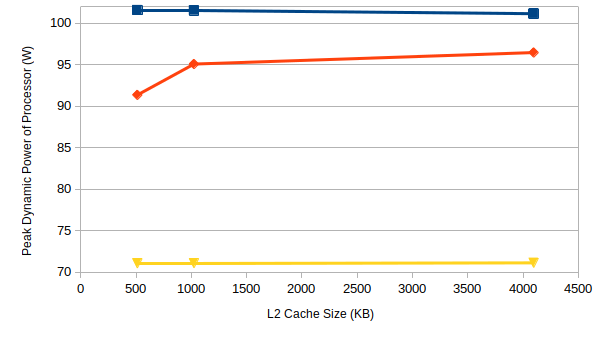
\includegraphics[width=1\textwidth]{output/L2SizeVProcPower.png}
                \caption{}
                \label{fig:peakdynamicplotsproc}
            \end{subfigure} &
            \begin{subfigure}{0.2\textwidth}
                \centering
                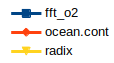
\includegraphics[width=1\textwidth]{output/colorLegend.png}
                % \caption{}
                \label{} 
            \end{subfigure} \\
            \begin{subfigure}{0.8\textwidth}
                \centering
                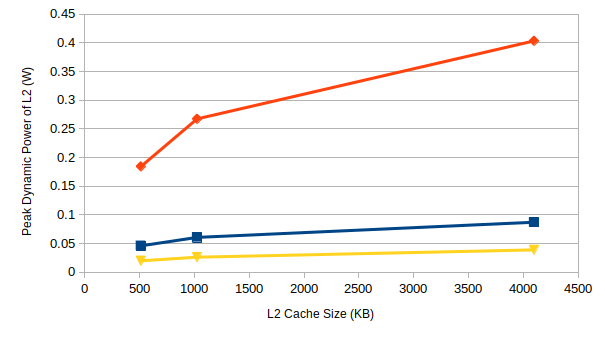
\includegraphics[width=1\textwidth]{output/L2SizeVL2Power.png}
                \caption{}
                \label{fig:peakdynamicplotsl2}
            \end{subfigure} & 
        \end{tabular}
        \caption{L2 cache sizes plotted against peak dynamic power of (a) the processor, and (b) the L2 cache, for each of the three benchmarks given in the legend.}
        \label{fig:peakdynamicplots}
    \end{figure}

    For each of the individual L2 cache sizes accross the three benchmarks, peak dynamic power (DP) of the processor (Fig. \ref{fig:peakdynamicplotsproc}) for \texttt{fft\_O2} always peaked higher than \texttt{ocean.cont} which always peaked higher than \texttt{radix}. Sweeping across the L2 cache size, \texttt{fft\_O2} DP always peaked higher than \texttt{radix} for the reasons it consumed more enery than \texttt{radix} discussed on the previous page. \texttt{fft\_O2} DP peaking higher than \texttt{ocean.cont} each time, though, even though \texttt{ocean.cont} consumed more total energy, may be due to \texttt{fft\_O2} having more branch instructions than the \texttt{ocean.cont} benchmark (see the yellow strip in the cpi-stacks in Fig. \ref{fig4MBcompare}). Things like speculative execution and missed branch predictions are costly in power, and those potentials may increase as branch insturction increase.

    For each of the individual L2 cache sizes accross the three benchmarks, peak DP of the L2 (Fig. \ref{fig:peakdynamicplotsl2}) was as expected, where no matter the L2 cache size, the \texttt{ocean.cont} always peaked higher thant \texttt{fft\_O2} which peaked higher than  \texttt{radix}. Looking back at Fig. \ref{fig4MBcompare.fft:power} - \ref{fig4MBcompare.radix:power}, this matches what we see, where in \texttt{ocean.cont}, the L2 consumed more energy than the L2 in \texttt{fft\_O2}, which consumed more energy than the L2 in \texttt{radix}. In Fig. \ref{fig4MBcompare.fft:cpi} - \ref{fig4MBcompare.radix:cpi}, we can also see that tests with more \texttt{mem-dram} instructions consumer more energy; in particular, \texttt{ocean.cont} spends a larger fraction of time on these instructions than any other, which we see \texttt{fft\_O2} spends almost equal time between \texttt{mem-dram} and \texttt{base} operations, which likely contributes to why it's L2 doesn't peak higher than that of \texttt{ocean.cont}.

   





    \clearpage
    %%%%%%%%%%%%%%%%%%%%%%%%%%%%%%%%%%%%%%%%%%%%%%%%%%%%%%%%%%%%%%%%%%%%%%%%


    \section{Performance Analysis}

        \begin{figure}[hbt!]
            \centering
            \begin{tabular}{cc}
                \begin{subfigure}{0.5\textwidth}
                    \centering
                    \includegraphics[width=1\textwidth]{output/fft_O2/L2SizeVipc.png}
                    \caption{}
                    \label{fig:ipcVsize.fft}
                \end{subfigure} &
                \begin{subfigure}{0.5\textwidth}
                    \centering
                    \includegraphics[width=1\textwidth]{output/ocean.cont/L2SizeVipc.png}
                    \caption{}
                    \label{fig:ipcVsize.ocean}
                \end{subfigure}
            \end{tabular}
        \end{figure}

        \begin{figure}[hbt!]\ContinuedFloat
            \centering
            \begin{tabular}{cc}
                \begin{subfigure}{0.5\textwidth}
                    \centering
                    \includegraphics[width=1\textwidth]{output/radix/L2SizeVipc.png}
                    \caption{}
                    \label{fig:ipcVsize.radix}
                \end{subfigure} &
                \begin{subfigure}{0.5\textwidth}
                    \centering
                    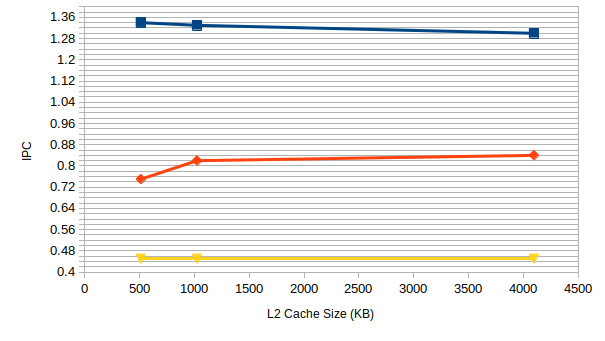
\includegraphics[width=1\textwidth]{output/L2SizeVipc2.png}
                    \caption{}
                    \label{fig:ipcVsize:all}
                \end{subfigure} 
            \end{tabular}
            \caption{L2 Cache Size vs. IPC plots for the (a) \texttt{fft\_O2} (blue), (b) \texttt{ocean.cont} (orange), and (c) \texttt{radix} (yellow) benchmarks; All plots are displayed together in Fig. \ref{fig:ipcVsize:all} in order to see the IPC across the three benchmarks for one L2 cache size.}
            \label{fig:ipcVsize}
        \end{figure}

        Fig. \ref{fig:ipcVsize} shows that L2 cache size affects IPC differently for each benchmark. Firstly, Fig. \ref{fig:ipcVsize:all} shows all the benchmarks together; for a given L2 size, \texttt{fft\_O2} has greater IPC than \texttt{ocean.cont}, which is greater than \texttt{radix}. \texttt{FTT} was already noted to be more optimized than \texttt{Radix}\cite{splash2}. It is surprising that given the lower energy stack and particular CPI stack for \texttt{radix} in Fig. \ref{fig4MBcompare}, that is has lower IPC than the other benchmarks; this may be due to inefficient sorting algorithms rather than the type of instructions it uses. Since it does not have much in ways of memory accessing instructions (Fig. (2-4)f), it makes sense that in Fig. \ref{fig:ipcVsize.radix}, the IPC doesn't change with the L2 cache size for \texttt{radix}. 
        
        In Fig. \ref{fig:ipcVsize.fft}, IPC decreases with L2 cache size for \texttt{fft\_O2}: Typically, we'd see that increasing total cache size improves miss rate\cite{book} (Appendix B), and therefore overall performance, yet IPC decreases with the L2 sweep. Since associativity and block sized remained the same across the sweep, this dip in performance with larger L2 could be the result of incurring a greater miss and hit access times for memory because it is larger. This is supported by the fact that in \texttt{fft\_O2}, the L2 consumes the most energy relative to the other components when L2 is 4 MB (Fig. \ref{fig4MBcompare.fft:power}), and that a substantial fraction of its time is spend on memory accessing instructions (Fig. \ref{fig4MBcompare.fft:cpi}). Penalties in memory access could be negatively affecting other performance. 
        

        Conversly, in Fig. \ref{fig:ipcVsize.ocean}, IPC increases with L2 cache size for \texttt{ocean.cont}: This benchmark probably does benefit from the improved miss rate of a larger total L2 cache size without incurring higher miss/hit penalty for accessing memory. \texttt{ocean.cont} operations lean heavily more on memory access instructions than the other benchmarks (Fig. (2-4)e), and at the larger 4 MB L2 cache size, more energy is consumed by L2 than any other component (Fig. \ref{fig4MBcompare.ocean.cont:power}). Differently than \texttt{fft\_O2}, DP peaks for L2 higher for \texttt{ocean.cont} than \texttt{fft\_O2} (Fig. \ref{fig:peakdynamicplotsl2}); so, by Amdahl's Law, improvemnts in L2 size would benefit performance in \texttt{ocean.cont} proportionally more than for \texttt{fft\_O2}.

    \section{Conclusion}
        Using the \texttt{SniperSim} tool, we were able to observe affects of L2 cache sizes across three benchmarks that each had observable differences between their CPI stacks. Unsurprisingly, as L2 size increased, so did it's energy consumption; across different benchmarks' performance, only those that had larger fractions on time with memory access operations were sensitive to the L2 sweep. A surprising result was that increasing the L2 cache size negatively affected IPC of the \texttt{fft\_O2} benchmark. If time permitted for more follow-up simulations, I suggest running these benchmarks with additional sweeps on cache associativity and block size. The current associativity of 8 may be high enough that is negatively affects performance in \texttt{fft\_O2} at the larger L2 cache size because of the cost of searching 8 ways in parallel, so I would expect it to improve for \texttt{fft\_O2}. If it gets low enough, it is likely to negatively impact performance for  \texttt{fft\_O2} and \texttt{ocean.cont}, because they have significant fraction of time spent doing memory access instructions, while all this won't affect IPC of \texttt{radix} just as it wasn't affect in the L2 cache size sweep. Likewise, it may be interesting to see a sweep of cache block size, because a too low or too high block size (range of about 16 to 256 byte) can both negatively impact performance for a particular total cache size\cite{book} (Appendix B). I would expect to see the IPC data to have a bell shape with a cache block size sweep. 

    \clearpage
    %%%%%%%%%%%%%%%%%%%%%%%%%%%%%%%%%%%%%%%%%%%%%%%%%%%%%%%%%%%%%%%%%%%%%%%%



    \section{Appendix: Post Processed Data (Figures and Output Values)}
    \label{appendix}

    \subsection{fft\_O2} %%%%%%%%%%%%%%%%%%%%%%%%%%%%%%%%%%%

        % \subsubsection{Simulation Output}%%%%%%%%%%%%%%%%%%%%%%%%%%%%%%%%%%%
        % % \begin{figure}[hbt!]
        %     \centering
        %     % \lstinputlisting{output/fft_O2/lab0L2-512KB/sim.out}
        %     % \renewcommand\mylstcaption{Example listing of code}
        %     \begin{mdlisting}
        %     % \lstinputlisting[language=csh, caption=\mylstcaption, label=lst:c1, xleftmargin=-2em]{output/fft_O2/lab0L2-512KB/sim.out}
        %     \lstinputlisting[language=csh, xleftmargin=-2em]{output/fft_O2/lab0L2-512KB/sim.out}
        %     \end{mdlisting}
        %     % \caption{}
        %     % \label{fig:fftO2:sim}
        % % \end{figure}

        % \clearpage
        
        \subsubsection{Power Results} %%%%%%%%%%%%%%%%%%%%%%%%%%%%%%%%%%%
        \begin{figure}[hbt!]
            \centering
            \begin{tabular}{cc}
                \begin{subfigure}{0.425\textwidth}
                    \centering
                    \includegraphics[width=1\textwidth]{output/fft_O2/lab0L2-512KB/power-chop.png}
                    \caption{}
                    \label{}
                \end{subfigure} &
                \begin{subfigure}{0.425\textwidth}
                    \centering
                    \includegraphics[width=1\textwidth]{output/fft_O2/lab0L2-1MB/power-chop.png}
                    \caption{}
                    \label{}
                \end{subfigure} \\
                \begin{subfigure}{0.425\textwidth}
                    \centering
                    \includegraphics[width=1\textwidth]{output/fft_O2/lab0L2-4MB/power-chop.png}
                    \caption{}
                    % \label{}
                \end{subfigure} &
                \begin{subfigure}{0.3\textwidth}
                    \centering
                    \includegraphics[width=1\textwidth]{output/fft_O2/lab0L2-4MB/power-legend.png}
                    % \caption{}
                    % \label{}
                \end{subfigure}
            \end{tabular}
            \caption{Power for core 0 in \texttt{fft\_O2} benchmark with L2 cache size of (a) 512 KB, (b) 1 MB, and (c) 4 MB.}
            \label{fig:fftO2:power}
        \end{figure}
        \clearpage

        \begin{figure}[hbt!]
            \centering
            \noindent\begin{subfigure}{0.75\textwidth}
            \lstinputlisting{output/fft_O2/lab0L2-512KB/power.out}
            \caption{}
            \end{subfigure}%

            \noindent\begin{subfigure}{0.75\textwidth}
            \lstinputlisting{output/fft_O2/lab0L2-1MB/power.out}
            \caption{}
            \end{subfigure}%
        \end{figure}
        \clearpage

        \begin{figure}[hbt!]\ContinuedFloat
            \centering
            \noindent\begin{subfigure}{0.75\textwidth}
            \lstinputlisting{output/fft_O2/lab0L2-4MB/power.out}
            \caption{}
            \end{subfigure}%
            \caption{Specific values for each components' power consumption (See. Fig. \ref{fig:fftO2:power}), for \texttt{fft\_O2} benchmark with L2 cache size of (a) 512 KB, (b) 1 MB, and (c) 4 MB.}
            \label{fig:fftO2:power-values}
        \end{figure}
        \clearpage

        \subsubsection{CPI Stacks} %%%%%%%%%%%%%%%%%%%%%%%%%%%%%%%%%%%
        \begin{figure}[hbt!]
            \centering
            \begin{tabular}{cc}
                \begin{subfigure}{0.4\textwidth}
                    \centering
                    \includegraphics[width=1\textwidth]{output/fft_O2/lab0L2-512KB/cpi-stack-chop.png}
                    \caption{}
                    \label{}
                \end{subfigure} &
                \begin{subfigure}{0.4\textwidth}
                    \centering
                    \includegraphics[width=1\textwidth]{output/fft_O2/lab0L2-1MB/cpi-stack-chop.png}
                    \caption{}
                    \label{}
                \end{subfigure} \\
                \begin{subfigure}{0.4\textwidth}
                    \centering
                    \includegraphics[width=1\textwidth]{output/fft_O2/lab0L2-4MB/cpi-stack-chop.png}
                    \caption{}
                    % \label{}
                \end{subfigure} &
                \begin{subfigure}{0.4\textwidth}
                    \centering
                    \includegraphics[width=1\textwidth]{output/fft_O2/lab0L2-4MB/cpi-stack-legend.png}
                    % \caption{}
                    % \label{}
                \end{subfigure}
            \end{tabular}
            \caption{CPI stack for \texttt{fft\_O2} benchmark with L2 cache size of (a) 512 KB, (b) 1 MB, and (c) 4 MB. Specific values for each components' fraction of time given in Fig. \ref{fig:fftO2:cpi-values}}
            \label{fig:fftO2:cpi-stack}
        \end{figure}
        \clearpage

        \begin{figure}[hbt!]
            \centering
            \noindent\begin{subfigure}{0.75\textwidth}
            \lstinputlisting{output/fft_O2/lab0L2-512KB/cpi-stack.out}
            \caption{}
            \end{subfigure}%

            \noindent\begin{subfigure}{0.75\textwidth}
            \lstinputlisting{output/fft_O2/lab0L2-1MB/cpi-stack.out}
            \caption{}
            \end{subfigure}%
        \end{figure}
        \clearpage

        \begin{figure}[hbt!]\ContinuedFloat
            \centering
            \noindent\begin{subfigure}{0.75\textwidth}
            \lstinputlisting{output/fft_O2/lab0L2-4MB/cpi-stack.out}
            \caption{}
            \end{subfigure}%
            \caption{Specific values for each components' CPI stack fraction of time (See. Fig. \ref{fig:fftO2:cpi-stack}), for \texttt{fft\_O2} benchmark with L2 cache size of (a) 512 KB, (b) 1 MB, and (c) 4 MB.}
            \label{fig:fftO2:cpi-values}
        \end{figure}

        \clearpage
    %%%%%%%%%%%%%%%%%%%%%%%%%%%%%%%%%%%%%%%%%%%%%%%%%%%%%%%%%%%%%%%%%%%%%%

    \subsection{ocean.cont} %%%%%%%%%%%%%%%%%%%%%%%%%%%%%%%%%%%
        \subsubsection{Power Results}
        \begin{figure}[hbt!]
            \centering
            \begin{tabular}{cc}
                \begin{subfigure}{0.425\textwidth}
                    \centering
                    \includegraphics[width=1\textwidth]{output/ocean.cont/lab0L2-512KB/power-chop.png}
                    \caption{}
                    \label{}
                \end{subfigure} &
                \begin{subfigure}{0.425\textwidth}
                    \centering
                    \includegraphics[width=1\textwidth]{output/ocean.cont/lab0L2-1MB/power-chop.png}
                    \caption{}
                    \label{}
                \end{subfigure} \\
                \begin{subfigure}{0.425\textwidth}
                    \centering
                    \includegraphics[width=1\textwidth]{output/ocean.cont/lab0L2-4MB/power-chop.png}
                    \caption{}
                    % \label{}
                \end{subfigure} &
                \begin{subfigure}{0.3\textwidth}
                    \centering
                    \includegraphics[width=1\textwidth]{output/ocean.cont/lab0L2-4MB/power-legend.png}
                    % \caption{}
                    % \label{}
                \end{subfigure}
            \end{tabular}
            \caption{Power for core 0 in \texttt{ocean.cont} benchmark with L2 cache size of (a) 512 KB, (b) 1 MB, and (c) 4 MB.}
            \label{fig:ocean.cont:power}
        \end{figure}
        \clearpage

        \begin{figure}[hbt!]
            \centering
            \noindent\begin{subfigure}{0.75\textwidth}
            \lstinputlisting{output/ocean.cont/lab0L2-512KB/power.out}
            \caption{}
            \end{subfigure}%

            \noindent\begin{subfigure}{0.75\textwidth}
            \lstinputlisting{output/ocean.cont/lab0L2-1MB/power.out}
            \caption{}
            \end{subfigure}%
        \end{figure}
        \clearpage

        \begin{figure}[hbt!]\ContinuedFloat
            \centering
            \noindent\begin{subfigure}{0.75\textwidth}
            \lstinputlisting{output/ocean.cont/lab0L2-4MB/power.out}
            \caption{}
            \end{subfigure}%
            \caption{Specific values for each components' power consumption (See. Fig. \ref{fig:ocean.cont:power}), for \texttt{ocean.cont} benchmark with L2 cache size of (a) 512 KB, (b) 1 MB, and (c) 4 MB.}
            \label{fig:ocean.cont:power-values}
        \end{figure}
        \clearpage

        \subsubsection{CPI Stacks} %%%%%%%%%%%%%%%%%%%%%%%%%%%%%%%%%%%

        \begin{figure}[hbt!]
            \centering
            \begin{tabular}{cc}
                \begin{subfigure}{0.4\textwidth}
                    \centering
                    \includegraphics[width=1\textwidth]{output/ocean.cont/lab0L2-512KB/cpi-stack-chop.png}
                    \caption{}
                    \label{}
                \end{subfigure} &
                \begin{subfigure}{0.4\textwidth}
                    \centering
                    \includegraphics[width=1\textwidth]{output/ocean.cont/lab0L2-1MB/cpi-stack-chop.png}
                    \caption{}
                    \label{}
                \end{subfigure} \\
                \begin{subfigure}{0.4\textwidth}
                    \centering
                    \includegraphics[width=1\textwidth]{output/ocean.cont/lab0L2-4MB/cpi-stack-chop.png}
                    \caption{}
                    \label{}
                \end{subfigure} &
                \begin{subfigure}{0.4\textwidth}
                    \centering
                    \includegraphics[width=1\textwidth]{output/ocean.cont/lab0L2-4MB/cpi-stack-legend.png}
                    % \caption{}
                    % \label{}
                \end{subfigure}
            \end{tabular}
            \caption{CPI stack for \texttt{ocean.cont} benchmark with L2 cache size of (a) 512 KB, (b) 1 MB, and (c) 4 MB. Specific values for each components' fraction of time given in Fig. \ref{fig:ocean.cont:cpi-values}}
            \label{fig:ocean.cont:cpi-stack}
        \end{figure}
        \clearpage

        \begin{figure}[hbt!]
            \centering
            \noindent\begin{subfigure}{1\textwidth}
                \lstinputlisting{output/ocean.cont/lab0L2-512KB/cpi-stack.out}
                \caption{}
            \end{subfigure}%

            \noindent\begin{subfigure}{1\textwidth}
                \lstinputlisting{output/ocean.cont/lab0L2-1MB/cpi-stack.out}
                \caption{}
            \end{subfigure}%
        \end{figure}
        \clearpage

        \begin{figure}[hbt!]
            \centering
            \noindent\begin{subfigure}{1\textwidth}
                \lstinputlisting{output/ocean.cont/lab0L2-4MB/cpi-stack.out}
                \caption{}
            \end{subfigure}%
            \caption{Specific values for each components' CPI stack fraction of time (See. Fig. \ref{fig:ocean.cont:cpi-stack}), for \texttt{ocean.cont} benchmark with L2 cache size of (a) 512 KB, (b) 1 MB, and (c) 4 MB.}
            \label{fig:ocean.cont:cpi-values}
        \end{figure}
        \clearpage
    %%%%%%%%%%%%%%%%%%%%%%%%%%%%%%%%%%%%%%%%%%%%%%%%%%%%%%%%%%%%%%%%%%%%%%


    \subsection{radix} %%%%%%%%%%%%%%%%%%%%%%%%%%%%%%%%%%%
        \subsubsection{Power Results}
        \begin{figure}[hbt!]
            \centering
            \begin{tabular}{cc}
                \begin{subfigure}{0.425\textwidth}
                    \centering
                    \includegraphics[width=1\textwidth]{output/radix/lab0L2-512KB/power-chop.png}
                    \caption{}
                    \label{}
                \end{subfigure} &
                \begin{subfigure}{0.425\textwidth}
                    \centering
                    \includegraphics[width=1\textwidth]{output/radix/lab0L2-1MB/power-chop.png}
                    \caption{}
                    \label{}
                \end{subfigure} \\
                \begin{subfigure}{0.425\textwidth}
                    \centering
                    \includegraphics[width=1\textwidth]{output/radix/lab0L2-4MB/power-chop.png}
                    \caption{}
                    % \label{}
                \end{subfigure} &
                \begin{subfigure}{0.3\textwidth}
                    \centering
                    \includegraphics[width=1\textwidth]{output/radix/lab0L2-4MB/power-legend.png}
                    % \caption{}
                    % \label{}
                \end{subfigure}
            \end{tabular}
            \caption{Power for core 0 in \texttt{radix} benchmark with L2 cache size of (a) 512 KB, (b) 1 MB, and (c) 4 MB.}
            \label{fig:radix:power}
        \end{figure}
        \clearpage

        \begin{figure}[hbt!]
            \centering
            \noindent\begin{subfigure}{0.75\textwidth}
            \lstinputlisting{output/radix/lab0L2-512KB/power.out}
            \caption{}
            \end{subfigure}%

            \noindent\begin{subfigure}{0.75\textwidth}
            \lstinputlisting{output/radix/lab0L2-1MB/power.out}
            \caption{}
            \end{subfigure}%
        \end{figure}
        \clearpage

        \begin{figure}[hbt!]\ContinuedFloat
            \centering
            \noindent\begin{subfigure}{0.75\textwidth}
            \lstinputlisting{output/radix/lab0L2-4MB/power.out}
            \caption{}
            \end{subfigure}%
            \caption{Specific values for each components' power consumption (See. Fig. \ref{fig:radix:power}), for \texttt{radix} benchmark with L2 cache size of (a) 512 KB, (b) 1 MB, and (c) 4 MB.}
            \label{fig:radix:power-values}
        \end{figure}
        \clearpage

        \subsubsection{CPI Stacks} %%%%%%%%%%%%%%%%%%%%%%%%%%%%%%%%%%%

        \begin{figure}[hbt!]
            \centering
            \begin{tabular}{cc}
                \begin{subfigure}{0.4\textwidth}
                    \centering
                    \includegraphics[width=1\textwidth]{output/radix/lab0L2-512KB/cpi-stack-chop.png}
                    \caption{}
                    \label{}
                \end{subfigure} &
                \begin{subfigure}{0.4\textwidth}
                    \centering
                    \includegraphics[width=1\textwidth]{output/radix/lab0L2-1MB/cpi-stack-chop.png}
                    \caption{}
                    \label{}
                \end{subfigure} \\
                \begin{subfigure}{0.4\textwidth}
                    \centering
                    \includegraphics[width=1\textwidth]{output/radix/lab0L2-4MB/cpi-stack-chop.png}
                    \caption{}
                    % \label{}
                \end{subfigure} &
                \begin{subfigure}{0.4\textwidth}
                    \centering
                    \includegraphics[width=1\textwidth]{output/radix/lab0L2-4MB/cpi-stack-legend.png}
                    % \caption{}
                    % \label{}
                \end{subfigure}
            \end{tabular}
            \caption{CPI stack for \texttt{radix} benchmark with L2 cache size of (a) 512 KB, (b) 1 MB, and (c) 4 MB. Specific values for each components' fraction of time given in Fig. \ref{fig:radix:cpi-values}}
            \label{fig:radix:cpi-stack}
        \end{figure}
        \clearpage

        \begin{figure}[hbt!]
            \centering
            \noindent\begin{subfigure}{0.75\textwidth}
            \lstinputlisting{output/radix/lab0L2-512KB/cpi-stack.out}
            \caption{}
            \end{subfigure}%

            \noindent\begin{subfigure}{0.75\textwidth}
            \lstinputlisting{output/radix/lab0L2-1MB/cpi-stack.out}
            \caption{}
            \end{subfigure}%
            % \pagebreak

            \noindent\begin{subfigure}{0.75\textwidth}
            \lstinputlisting{output/radix/lab0L2-4MB/cpi-stack.out}
            \caption{}
            \end{subfigure}%
            \caption{Specific values for each components' CPI stack fraction of time (See. Fig. \ref{fig:radix:cpi-stack}), for \texttt{radix} benchmark with L2 cache size of (a) 512 KB, (b) 1 MB, and (c) 4 MB.}
            \label{fig:radix:cpi-values}
        \end{figure}
        \clearpage
    %%%%%%%%%%%%%%%%%%%%%%%%%%%%%%%%%%%%%%%%%%%%%%%%%%%%%%%%%%%%%%%%%%%%%%



    % \begin{thebibliography}{1}
    %     \bibitem[1]{sniper}\href{https://snipersim.org/w/The_Sniper_Multi-Core_Simulator}{The Sniper Multi-Core Simulator}
    %     \bibitem[2]{parallel}O. Tange (2011): \href{https://www.gnu.org/software/parallel/parallel_tutorial.html}{GNU Parallel}  - The Command-Line Power Tool
    %     \bibitem[3]{oh}Mark, Robert, and Bharat's office hours
    %     \bibitem[4]{splash2}S. C. Woo, M. Ohara, E. Torrie, J. P. Singh and A. Gupta, \href{https://citeseerx.ist.psu.edu/viewdoc/download?doi=10.1.1.48.2356&rep=rep1&type=pdf}{The SPLASH-2 Programs: Characterizaion and Methodological Considerations}, Proceedings 22nd Annual International Symposium on Computer Architecture, Santa Margherita Ligure, Italy, 1995, pp. 24-36
    % \end{thebibliography}
    % \pagebreak

    % \section{Others}

    

\end{document}